\section[1978年高考数学试卷及答案(全国卷)理科]{1978年普通高等学校招生考试(全国卷)\\\Huge{理科数学}}
\begin{questions}
	\question
	\begin{parts}
		\part[4] 分解因式:$x^2 - 4xy + 4y^2 - 4z^2$.

			\begin{solution}
				\begin{align*}
					 & = (x-2y)^2 - 4z^2    \\
					 & = (x-2y+2z)(x-2y-2z)
				\end{align*}
			\end{solution}

		\part[4] 已知正方形的边长为$a$,求侧面积等于这个正方形的面积,高等于这个正方形边长的直圆柱体的体积.

			\begin{solution}
				设直圆柱体的直径为$r$,则有侧面积:
				\begin{equation*}
					S_侧 = 2\pi{r}a
				\end{equation*}
				因为直圆柱体的侧面积等于正方形的面积,因此有:
				\begin{align*}
					2\pi{r}a = a^2 \\
					r = \frac{a}{2\pi}
				\end{align*}
				所以可得直圆柱体的体积为:
				\begin{align*}
					V & = \pi{r^2}a               \\
					  & = \pi \frac{a^2}{4\pi^2}a \\
					  & = \frac{a^3}{4\pi}
				\end{align*}
			\end{solution}

		\part[4] 求函数$y=\sqrt{\lg(2+x)}$的定义域.

			\begin{solution}
				\begin{cenum}
					\item 由$\lg(2+x) \geqslant 0$得:
					      \begin{align*}
						      2+x \geqslant 1 \\
						      x \geqslant -1
					      \end{align*}

					      \begin{center}
						      \begin{tikzpicture}
							      \begin{axis}[
									      xmin = -4, xmax = 4,
									      ticks=both
								      ]
								      \addplot[domain=-3:3, blue!70, thick]{log10(x+2)};
								      \addlegendentry{$\lg(x+2)$}
							      \end{axis}
						      \end{tikzpicture}
					      \end{center}

					\item 由$2+x > 0$得:
					      \begin{equation*}
						      x > -2
					      \end{equation*}
					\item 综上,函数的定义域为$\{x|x\geqslant-1\}$.

				\end{cenum}
			\end{solution}

		\part[4] 不查表求$\cos\ang{80}\cos\ang{35} + \cos\ang{10}\cos\ang{55}$的值.
			\begin{solution}
				\begin{align*}
					 & = \cos\ang{80}\cos\ang{35} + \sin\ang{80}\sin\ang{35} \\
					 & = \cos(\ang{80} - \ang{35})                           \\
					 & = \cos\ang{45}                                        \\
					 & = \frac{\sqrt{2}}{2}
				\end{align*}
			\end{solution}
		\part[4] 化简: $\displaystyle\left( \frac14 \right)^{-\frac12}\cdot
				\frac{(\sqrt{4ab^{-1}})^3}{(0.1)^{-2}(a^3b^{-4})^{\frac12}}$.
			\begin{solution}
				\begin{align*}
					 & = 2 \cdot \frac{(4ab^{-1})^{\frac32}}{100a^\frac32b^{-2}}                 \\
					 & = 2 \cdot \frac{4^{\frac32}a^{\frac32}b^{-\frac32}}{100a^{\frac32}b^{-2}} \\
					 & = 2 \cdot \frac{8\sqrt{b}}{100}                                           \\
					 & = \frac4{25}\sqrt{b}
				\end{align*}
			\end{solution}
	\end{parts}

	\question[14] 已知方程$kx^2 + y^2 =
		4$,其中$k$为实数,对于不同范围的$k$值,分别指出方程所代表图形的类型,并画出显示其数量特征的草图.

	\begin{solution}
		\begin{penum}
			\item $k = 0$时,$y=\pm2$,这是两条平行于$x$轴的直线;
			      \begin{center}
				      \begin{tikzpicture}
					      \begin{axis}[xmin=-3, xmax=3, ymax=3, ymin=-3]
						      \addplot[domain=-2:2, green!50!blue, thick]{2};
						      \addplot[domain=-2:2, red!50!blue, thick]{-2};
						      \addlegendentry{$y=2$}
						      \addlegendentry{$y=-2$}
						      \node[below left] at (0,2) {$2$};
						      \node[below left] at (0,-2) {$-2$};
					      \end{axis}
				      \end{tikzpicture}
			      \end{center}

			\item $k > 0$时,图形是半轴分别为$\frac{2}{\sqrt{k}}$和$2$的椭圆,其中当$k = 1$时,长短轴相等形状为圆形;
			\item $k < 0$时,图形是双曲线.
			      \begin{center}
				      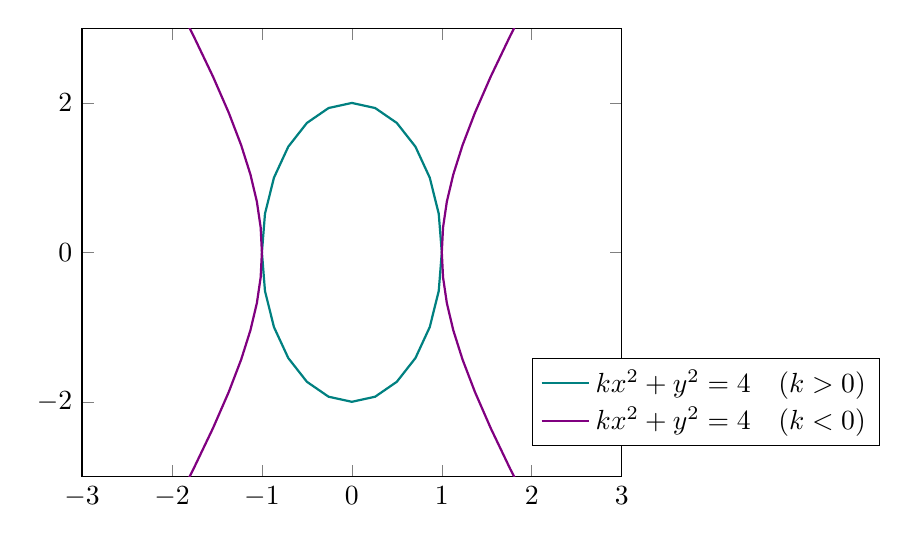
\begin{tikzpicture}
					      \begin{axis}[xmin=-3, xmax=3, ymax=3, ymin=-3,
							      legend style={at={(axis cs:2,-2)}, anchor=west}]
						      \addplot[domain=0:360, green!50!blue, thick]({cos(x)}, {2*sin(x)});
						      \addlegendentry{$kx^2 + y^2 = 4 \quad(k>0)$}
						      \addlegendentry{$kx^2 + y^2 = 4 \quad(k<0)$}
						      \addplot[domain=-2:2, red!50!blue, thick]({cosh(x)}, {2*sinh(x)});
						      \addplot[domain=-2:2, red!50!blue, thick]({-cosh(x)}, {2*sinh(x)});
					      \end{axis}
				      \end{tikzpicture}
			      \end{center}
		\end{penum}
	\end{solution}

	\question[14] 如图,$AB$是半圆的直径,$C$是半圆上的一点,直线$MN$切半圆于$C$点,$AM\perp MN$于$M$点,$CD\perp
		MN$于$N$点,$CD\perp AB$于$D$点,求证:
	\begin{penum}
		\item $CD=CM=CN$;
		\item $CD^2=AM\cdot BN$.
	\end{penum}
	\begin{center}
		\begin{tikzpicture}[scale=1.5]
			\def\pangle{55}
			\coordinate(o) at (0,0);
			\coordinate(c) at (\pangle:1);
			\coordinate(a) at (-1,0);
			\coordinate(b) at (1,0);
			\coordinate(d) at ($(a)!(c)!(b)$);
			\coordinate(t) at ({1/cos(\pangle)}, 0);
			\coordinate(m) at ($(c)!(a)!(t)$);
			\coordinate(n) at ($(c)!(b)!(t)$);
			\draw (a) arc [start angle=180, end angle=0, radius=1];
			\draw (a) -- (b) (c) -- (d) (a) -- (m) -- (n) -- (b);
			\draw (m)node[above]{$M$} (c) node[above]{$C$} (n) node[above]{$N$} (a)node[below left]{$A$} (d)node[below]{$D$}
			(b)node[below right]{$B$};

		\end{tikzpicture}
	\end{center}

	\begin{proofsolution}
		\begin{center}
			\begin{tikzpicture}[scale=1.5]
				\def\pangle{55}
				\coordinate(o) at (0,0);
				\coordinate(c) at (\pangle:1);
				\coordinate(a) at (-1,0);
				\coordinate(b) at (1,0);
				\coordinate(d) at ($(a)!(c)!(b)$);
				\coordinate(t) at ({1/cos(\pangle)}, 0);
				\coordinate(m) at ($(c)!(a)!(t)$);
				\coordinate(n) at ($(c)!(b)!(t)$);
				\draw (a) arc [start angle=180, end angle=0, radius=1];
				\draw (a) -- (b) (c) -- (d) (a) -- (m) -- (n) -- (b);
				\draw (m)node[above]{$M$} (c) node[above]{$C$} (n) node[above]{$N$} (a)node[below left]{$A$} (d)node[below]{$D$}
				(b)node[below right]{$B$} (o) node[below]{$O$};
				\draw[dashed, blue] (o) -- (c) -- (a) (b) -- (c);

				\draw[angle radius=10pt, red] pic[draw]{right angle=n--m--a} pic[draw]{right angle=n--c--o} pic[draw]{right
						angle=m--n--b};

			\end{tikzpicture}
		\end{center}
		\begin{penum}
			\item
			      \begin{cenum}
				      \item 连接圆心$O$与$C$点.
				            \begin{align*}
					             & \because AM \perp MN \land BN \perp MN  \land OC \perp MN \\
					             & \therefore AM \parallel BN \parallel OC                   \\
					             & \because AO = BO                                          \\
					             & \therefore MC = CN
				            \end{align*}
				      \item	连接$AC$.
				            \begin{align*}
					             & \because AO = OC                                            \\
					             & \therefore \angle{OAC} = \angle{OCA}                        \\
					             & \because AM \parallel CO                                    \\
					             & \therefore \angle{MAC} = \angle{ACO}                        \\
					             & \therefore \angle{DAC} = \angle{MAC}                        \\
					             & \because \angle{AMC} = \angle{ADC} = \ang{90} \land AC = AC \\
					             & \therefore \triangle{ACM} \cong \triangle{ACD}              \\
					             & \therefore MC = CD                                          \\
					             & \therefore MC = CN = CD
				            \end{align*}
			      \end{cenum}
			\item 连接$BC$.
			      \begin{align*}
				       & \because \angle{CDB} = \angle{CNB} = \ang{90} \land CD = CN \land CB = CB                   \\
				       & \therefore \triangle{BDC} \cong \triangle{BNC}                                              \\
				       & \therefore BD = BN                                                                          \\
				       & \because \angle{BCD} = \angle{CAB} = \angle{CAM} \land \angle{AMC} = \angle{CDB} = \ang{90} \\
				       & \therefore \triangle{AMC} \sim \triangle{CDB}                                               \\
				       & \therefore \frac{AM}{MC} = \frac{CD}{DB}                                                    \\
				       & \therefore \frac{AM}{CD} = \frac{CD}{BN}                                                    \\
				       & \therefore CD^2 = AM\cdot BN
			      \end{align*}
		\end{penum}
	\end{proofsolution}

	\question[12] 已知$\log_{18}9=a\,(a\neq2), 18^b=5$,求$\log_{36}45$.

	\begin{solution}
		由$18^b=5$得
		\begin{equation*}
			b = \log_{18}5
		\end{equation*}
		则有:
		\begin{equation*}
			a + b = \log_{18}{45}
		\end{equation*}
		根据换底公式有:
		\begin{equation*}
			\log_{18}{45} = \frac{\log_{36}{45}}{\log_{36}{18}}
		\end{equation*}
		则有:
		\begin{align*}
			\log_{36}{45} & = \log_{18}{45}\cdot \log_{36}{18}         \\
			              & = (a+b)\log_{36}{18}                       \\
			              & = (a+b)\frac{\log_{18}{18}}{\log_{18}{36}} \\
			              & = (a+b)\frac1{1+\log_{18}2}
		\end{align*}
		由$\log_{18}{9} = a$得:
		\begin{align*}
			\log_{18}9 & = \log_{18}\frac{18}{2}    \\
			           & = \log_{18}18 - \log_{18}2 \\
			           & = 1 - \log_{18}{2}         \\
			           & = a
		\end{align*}
		则有
		\begin{equation*}
			\log_{18}2 = 1 - a
		\end{equation*}

		所以有:
		\begin{equation*}
			\log_{36}{45} = \frac{a+b}{2-a}
		\end{equation*}

	\end{solution}

	\question[20] 已知$\triangle{ABC}$的三个内角的大小成等差数列,$\tan{A}\tan{C}=2+\sqrt{3}$,求角$A,B,C$的大小.又已知顶点$C$的对边$c$上的高等于$4\sqrt{3}$,求三角形各边$a,b,c$的长.(提示:必要时可验证$(1+\sqrt{3})^2=4+2\sqrt{3}$)

	\begin{solution}
		设$\angle{B}=\beta$,则角$A,B,C$可以分别表示为$\beta-\delta, \beta, \beta + \delta$,可知$\beta=\ang{60},
			\angle{A}+\angle{C} = \ang{120}$.

		因为有
		\begin{equation*}
			\tan{A}\tan{C}  = \frac{\sin{A}}{\cos{A}}\cdot\frac{\sin{C}}{\cos{C}}
		\end{equation*}
		所以得
		\begin{align*}
			\sin{A}\sin{C} = (2+\sqrt{3})\cos{A}\cos{C} \\
			(1+\sqrt{3})\cos{A}\cos{C} + \cos{A}\cos{C} - \sin{A}\sin{C} = 0
		\end{align*}
		根据和角公式可得
		\begin{align*}
			(1+\sqrt{3})\cos{A}\cos{C} + \cos(A+C)= 0 \\
			\cos{A}\cos{C} = \frac{\sqrt{3}-1}{4}
		\end{align*}
		根据余弦积化和差公式可得
		\begin{align*}
			\cos{A}\cos{C} & = \frac12[\cos(A+C)+\cos(A-C)]                        \\
			               & = -\frac14 + \frac12\cos(A-C)  = \frac{\sqrt{3}-1}{4}
		\end{align*}
		可得
		\begin{math}
			\cos(A-C) = \frac{\sqrt{3}}{2}
		\end{math}
		所以$A-C=\pm\ang{30}$.
		\begin{penum}
			\item $A-C=\ang{30}$则有$A=\ang{75}, C=\ang{45}$.
			      \begin{center}
				      \begin{tikzpicture}
					      \coordinate(a) at (0,0);
					      \coordinate(b) at (3,0);
					      \coordinate(a1) at (75:5);
					      \coordinate(b1) at ([xshift=3cm]120:5);
					      \coordinate(c) at (intersection of a--a1 and b--b1);
					      \coordinate(d) at ($(a)!(c)!(b)$);

					      \draw (a) -- (b) -- (c) -- cycle;
					      \draw[dashed, blue] (c) -- (d);
					      \draw (a)node[below]{$A$} (b) node[below]{$B$} (c)node[above]{$C$} (d) node[below]{$D$};

				      \end{tikzpicture}
			      \end{center}
			      根据条件可知$CD=4\sqrt{3}$,可以计算出$a=BC=8$,根据正弦定理有:
			      \begin{equation*}
				      \frac{a}{\sin\ang{75}} = \frac{b}{\sin\ang{60}} = \frac{c}{\sin\ang{45}}
			      \end{equation*}
			      应用和角公式来计算$\sin\ang{75}$:
			      \begin{align*}
				      \sin\ang{75} & = \sin(\ang{45}+\ang{30})                                                    \\
				                   & = \sin\ang{45}\cos\ang{30} + \cos\ang{45}\sin\ang{30}                        \\
				                   & = \frac{\sqrt{2}}{2}\cdot\frac{\sqrt{3}}{2} + \frac{\sqrt{2}}{2}\cdot\frac12 \\
				                   & = \frac{\sqrt{6} + \sqrt{2}}{4}
			      \end{align*}
			      则可以分别计算出:
			      \begin{align*}
				       & b = \frac{\sqrt{3}}{2}\cdot \frac{8}{\frac{\sqrt{6}+\sqrt{2}}{4}} = 4(3\sqrt{2} - \sqrt{6}) \\
				       & c = \frac{\sqrt{2}}{2}\cdot\frac{8}{\frac{\sqrt{6} + \sqrt{2}}{4}} = 8(\sqrt{3} - 1)
			      \end{align*}

			\item $A-C=-\ang{30}$则有$A=\ang{45}, C=\ang{75}$.
			      \begin{center}
				      \begin{tikzpicture}
					      \coordinate(a) at (0,0);
					      \coordinate(b) at (3,0);
					      \coordinate(a1) at (45:5);
					      \coordinate(b1) at ([xshift=3cm]120:5);
					      \coordinate(c) at (intersection of a--a1 and b--b1);
					      \coordinate(d) at ($(a)!(c)!(b)$);

					      \draw (a) -- (b) -- (c) -- cycle;
					      \draw[dashed, blue] (c) -- (d);
					      \draw (a)node[below]{$A$} (b) node[below]{$B$} (c)node[above]{$C$} (d) node[below]{$D$};

				      \end{tikzpicture}
			      \end{center}
			      根据条件可以简单计算出$a=8, b=4\sqrt{6}, c=2\sqrt{3}+4\sqrt{3}=6\sqrt{3}$.
		\end{penum}
	\end{solution}

	\question[20] 已知$\alpha,\beta$为锐角,$3\sin^2\alpha + 2\sin^2\beta=1, 3\sin2\alpha - 2\sin2\beta
		=0$.求证:$\alpha+2\beta=\frac{\pi}2.$

	\begin{proofsolution}
		由和角公式和倍角公式可得:
		\begin{align*}
			\sin(\alpha + 2\beta) & = \sin\alpha\cos2\beta + \cos\alpha\sin2\beta                      \\
			                      & = \sin\alpha(1 - 2\sin^2\beta) + \cos\alpha\cdot\frac32\sin2\alpha \\
			                      & = 3\sin^3\alpha  + 3\sin\alpha\cos^2\alpha                         \\
			                      & = 3\sin\alpha(\sin^2\alpha + \cos^2\alpha)                         \\
			                      & = 3\sin\alpha
		\end{align*}
		将$3\sin^2\alpha + 2\sin^2\beta=1$转换为$3\sin^2\alpha=\cos2\beta$并两边平方可得:
		\begin{equation*}
			9\sin^4\alpha = \cos^2{2\beta} \tag{1}
		\end{equation*}
		将$3\sin2\alpha-2\sin2\beta=0$移项得$3\sin2\alpha=2\sin2\beta$并两边平方可得:
		\begin{align*}
			 & 9\sin^2(2\alpha)  = 4\sin^22\beta               \\
			 & 9\sin^2(2\alpha)  = 4(1-\cos^22\beta)           \\
			 & \cos^22\beta = 1 - \frac94\sin^22\alpha \tag{2}
		\end{align*}
		结合式(1)和式(2)有:
		\begin{align*}
			 & 9\sin^4\alpha = 1 - \frac94\sin^22\alpha                 \\
			 & 36\sin^4\alpha = 4 - 9(1-\cos^22\alpha)                  \\
			 & 36\sin^4\alpha = 4 - 9[1-(1-2\sin^2\alpha)^2]            \\
			 & 36\sin^4\alpha = 4 - 9(1-1+4\sin^2\alpha -4\sin^4\alpha) \\
			 & 36\sin^4\alpha = 4 - 36\sin^2\alpha + 36\sin^4\alpha     \\
			 & \sin^2\alpha = \frac19
		\end{align*}
		又因为$\alpha$是锐角,所以$\sin\alpha=\frac13$.

		由此可得$\sin(\alpha+2\beta) = 1$, 所以$\alpha+2\beta=\frac{\pi}{2}$.
	\end{proofsolution}

	\question 已知函数$y=x^2 + (2m+1)x + m^2 - 1\, (m\text{为实数})$.
	\begin{penum}
		\item $m$是什么数值时,$y$的极值是$0$?
		\item
		      求证:不论$m$是什么数值时,函数图像(即抛物线)的顶点都在同一条直线$L_1$上,画出$m=-1,0,1$时抛物线的草图,来检验这个结论;
		\item
		      平行于$L_1$的直线中,哪些与抛物线相交,哪些不相交?求证:任一条平行于$L_1$而与抛物线相交的直线,被各抛物线裁出的线段都相等.
	\end{penum}

	\begin{solution}
		\begin{penum}
			\item 由抛物线的性质可知在$x=-\frac{2m+1}{2}$时有极值,代入函数中有:
			      \begin{align*}
				      y & = (-\frac{2m+1}{2})^2 - (2m+1)\frac{2m+1}{2} + m^2 - 1 \\
				        & = \frac{(2m+1)^2}{4} - \frac{(2m+1)^2}{2} + m^2 - 1    \\
				        & = \frac{4m^2 - 4 - 4m^2 - 4m - 1}{4}                   \\
				        & = -m - \frac54
			      \end{align*}
			      所以当$m=-\frac54$时极值为零.
			\item 联解顶点坐标的方程组
			      \begin{math}
				      \begin{cases}
					      x = -\frac{2m+1}{2} \\
					      y = -m - \frac54
				      \end{cases}
			      \end{math}
			      可得:
			      \begin{equation*}
				      y = x - \frac34
			      \end{equation*}
			      所以顶点在直线$y=x - \frac34$上.

			      \begin{center}
				      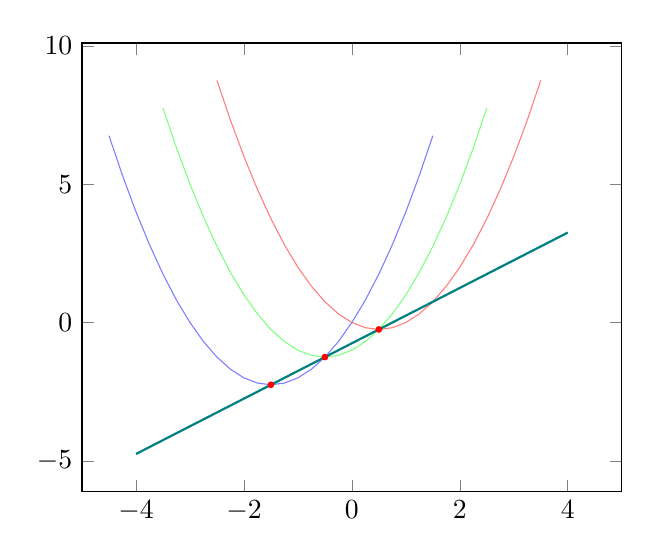
\begin{tikzpicture}
					      \begin{axis}[
							      xmin=-5, xmax=5
						      ]
						      \addplot[domain=-2.5:3.5, red!50]{x^2 - x};
						      \addplot[domain=-3.5:2.5, green!50]{x^2 + x - 1};
						      \addplot[domain=-4.5:1.5, blue!50]{x^2 + 3*x};
						      \addplot[domain=-4:4, green!50!blue, thick]{x - 3/4};
						      \draw[fill=red, red](0.5,-0.25)circle(1pt) (-.5,-1.25)circle(1pt) (-1.5, -2.25)circle(1pt);
					      \end{axis}
				      \end{tikzpicture}
			      \end{center}

			\item 设平行于$L_1$的直线方程为$y=x + b$,联解抛物线与直线的方程组
			      \begin{equation*}
				      \begin{cases}
					      y=x^2 + (2m+1)x + m^2 - 1 \\
					      y = x + b
				      \end{cases}
			      \end{equation*}
			      可得:
			      \begin{equation*}
				      x^2 + 2mx + m^2 - b - 1 = 0
			      \end{equation*}
			      当方程有两个相同的根时直线与抛物线相切,即方程的判别式$\Delta=0$时.
			      \begin{align*}
				      \Delta & = (2m)^2 - 4(m^2 - b - 1) \\
				             & = 4m^2 - 4m^2 + b + 1     \\
				             & = b + 1 = 0
			      \end{align*}
			      则当$b\geqslant-1$时与抛物线有相交,当$b<-1$时与抛物线没有交点.

			      当$b\geqslant-1$时求解交点的坐标:
			      \begin{equation*}
				      x_1,x_2 = \frac{-2m \pm \sqrt{b + 1}}{2}
			      \end{equation*}
			      对应的$y$坐标为:
			      \begin{align*}
				      y_1,y_2 = \frac{-2m \pm \sqrt{b + 1}}{2} + b
			      \end{align*}
			      交点之间的距离$l$为:
			      \begin{align*}
				      l & = \sqrt{(x_1 - x_2)^2 + (y_1 - y_2)^2} \\
				        & = \sqrt{b + 1 + b + 1}                 \\
				        & = \sqrt{2b + 2}
			      \end{align*}
			      所以与抛物线有交点的情况下直线被抛物线裁出的线段都相等(与$m$无关).

		\end{penum}
	\end{solution}

\end{questions}
